\section{Method calls}
\label{sec-optimisations-method-calls}

Finally, we will look at the overhead caused by method calls. In native code, the smallest function call only has 8 cycles of overhead for a \mycode{CALL} and \mycode{RET}, and some \mycode{MOV}s may be needed to move the parameters to the right registers. More complicated functions may spend up to 76 cycles saving and restoring call-saved registers. As we have seen in Section \ref{sec-overhead-method-call}, in Java a considerable amount of state needs to be initialised. For the simplest method call this takes about 550 cycles, and this increases further for large methods with many parameters.

When we look at the methods in a programme, we typically see a spectrum from a limited number of large methods at the base of the call tree that take a long time to complete and are only called a few times, to small (near-)leaf methods that are fast and frequently called. Figure \ref{fig-coremark-method-calls-vs-duration} shows this spectrum for the CoreMark benchmark.

For the slow methods at the base, the impact of the method call is not very significant for the overall execution time and we can afford to take the 550 cycles penalty. However, as we get closer to the leaf methods, the number of calls increases, as does the impact on the overall performance.

At the very end of this spectrum we have tiny helper functions that may be inlined. However, this is only possible for small methods, or methods called from a single place. In CoreMark's case, \mycode{ee\_isdigit} was small enough to inline. When we inline larger methods, the tradeoff is an increase in code size. So we have a problem in the middle of the spectrum: methods that are too large to inline, but called often enough for the method call overhead to have a significant impact the overall performance.

\subsection{Lightweight methods}
For these cases we introduce a new type of method call: lightweight methods. These methods differ from normal methods in two ways:
\begin{itemize}
	\item We do not create a stack frame for lightweight methods, but use the caller's frame.
	\item Parameters are passed on the stack, rather than in local variables.
\end{itemize}

\begin{figure}
\centering
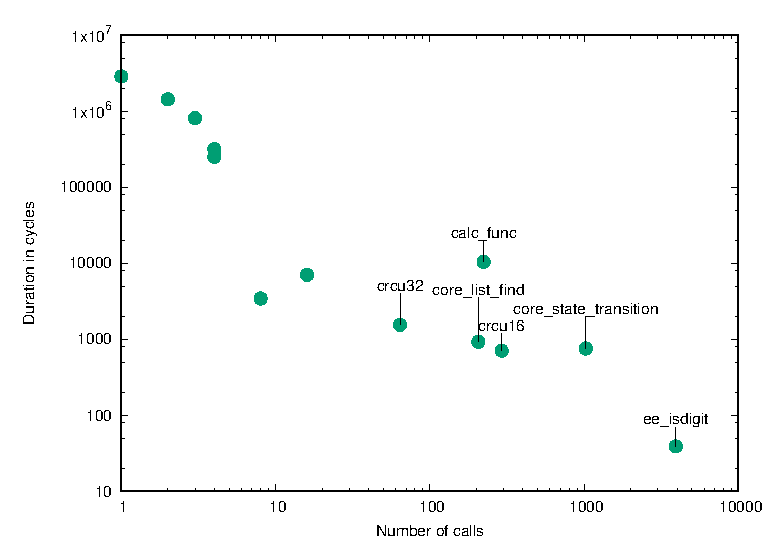
\includegraphics[width=.5\linewidth]{method-calls-vs-duration.eps}
\caption{CoreMark method calls vs duration with logarithmic scales}
\label{fig-coremark-method-calls-vs-duration}
\end{figure}

Lightweight methods give us third choice, in between a normal method call and method inlining. When calling a lightweight method, we directly \mycode{CALL} the method's code. We bypass the VM completely, reusing the caller's stack frame, and leaving the parameters on the (caller's) stack. In effect, the lightweight method behaves similar to inlined code, but since we can \mycode{CALL} it from multiple places, we do not incur the code size overhead of duplicating large inlined methods.

Because the method will be called from multiple locations which may have different cache states, we do have to flush the stack cache to memory before a call. This results in slightly more overhead than for inlined code, but much less than for a normal method call.

As an example, consider the simple \mycode{isOdd} method in Listing \ref{lst-lightweight-stack-only}:

\begin{listing}
\centering
\begin{minipage}[t]{0.32\textwidth}
\centering
\begin{minted}{java}
// JAVA

public static boolean
          isOdd (short a)
{
  return (a & (short)1)==1;
}
\end{minted}
\end{minipage}\hfill
\begin{minipage}[t]{0.29\textwidth}
\centering
\begin{minted}{java}
// NORMAL METHOD
//              (Stack)
SLOAD_0         (Int)
SCONST_1        (Int,Int)
SAND            (Int)
SRETURN         ()
\end{minted}
\end{minipage}\hfill
\begin{minipage}[t]{0.29\textwidth}
\centering
\begin{minted}{java}
// LIGHTWEIGHT METHOD
//              (Stack)
SCONST_1        (Int,Int)
SAND            (Int)
SRETURN         ()
\end{minted}
\end{minipage}
\caption{Simple, stack-only lightweight method example}
\label{lst-lightweight-stack-only}
\end{listing}

The normal implementation has a single local variable. It expects the parameter to be stored there and the stack to be empty when we enter the method. In contrast, the lightweight method does not have any local variables and expects the parameter to be on the stack.

We added a new instruction, \mycode{INVOKELIGHT}, to call lightweight methods. In the bottom half of Listing \ref{lst-comparison-lightweight-and-normal-invocation} we see how \mycode{INVOKELIGHT} and \mycode{INVOKESTATIC} are translated to native code. Both first flush the stack cache to memory. After that, the lightweight method can directly call the implementation of \mycode{isOdd}, while the native version first saves the stack pointers, and then enters an expensive call into the VM to setup a stack frame for \mycode{isOdd}, which in turn will call the actual method.

\begin{listing}
\centering
\begin{minipage}[t]{0.5\textwidth}
\centering
\begin{minted}{java}
// NORMAL INVOCATION
// INVOKESTATIC isOdd:
    push r25        // Flush the cache
    push r24
    call &preinvoke // Save X and SP
    ldi r22, 253    // Set parameters
    ldi r23, 2      //  for callMethod
    ldi r24, 21
    ldi r20, 64
    ldi r21, 42
    ldi r18, 13
    ldi r19, 0
    ldi r25, 2
    call &callMethod // Call to VM
    call &postinvoke // Restore X and SP
\end{minted}
\end{minipage}\hfill
\begin{minipage}[t]{0.45\textwidth}
\centering
\begin{minted}[linenos=false]{java}
// LIGHTWEIGHT INVOCATION
// INVOKELIGHT isOdd:
    push r25      // Flush the cache
    push r24
    call &isOdd
\end{minted}
\end{minipage}
\caption{Comparison of lightweight and normal method invocation}
\label{lst-comparison-lightweight-and-normal-invocation}
\end{listing}

\subsubsection{Local variables}
The lightweight implementation of the \mycode{isOdd} example only needs to process the values that are on the stack, but this is only possible for the smallest methods. If we want a lightweight method to be able to use local variables, we need to reserve space for them in the caller's stack frame, equal to the maximum number of slots needed by all the lightweight methods it may call.

In our AOT compiled code, we use the ATmega's Y register to point the start of a method's local variables. To call a lightweight method with local variables, the caller only needs to shift Y up to the region reserved for lightweight method variables before doing the \mycode{CALL}. The lightweight method can then access its locals as if it were a normal method.

\subsubsection{Nested calls}
A final extension is to allow for nested calls. While frequently called leaf methods benefit the most from lightweight methods, there are many cases where it is useful for lightweight methods to call other lightweight methods. A good example from the CoreMark benchmark is the 16-bit \mycode{crcu16} function, which is implemented as two calls to \mycode{crcu8}. While \mycode{crcu8} is the most critical, there is still one call to \mycode{crcu16} for every two to \mycode{crcu8}.

So far we have not discussed how to handle the return address in a lightweight method. Our AOT compiler uses the native stack to store JVM integer stack value, which means the operands to a lightweight method will be on the native stack. But when we do a \mycode{CALL}, the return address is put on the stack, covering the method parameters.

For leaf methods, the lightweight method will first pop the return address into two fixed registers, and avoid using these register for stack caching. When the method returns, the return address is pushed back onto the stack before the \mycode{RET} instruction.

For lightweight methods that will call another lightweight method, the return value is also popped from the stack, but instead of leaving it in the fixed register, where it would be overwritten by the nested call, we save it in the first local variable slot and increment Y to skip this slot. Since each lightweight method has its own block of locals, we can nest calls as deeply as we want.

This difference in method prologue and epilogue is the only difference in the way the VM generates code for a lightweight method, all JVM instructions can then be translated the same way as for a normal method.

\subsubsection{Stack frame layout}
A normal method that invokes a possible string of lightweight methods, needs to save space for this in its stack frame. How much space it needs to reserve can be determined by the infuser at compile time, and this information is added to the method descriptor.

% For each method the number of locals is known by the infuser. If it is a lightweight method that will call another lightweight, one extra slot is reserved for the return address. In addition, each method needs to reserve the maximum number of extra slots required for of any lightweight method it may call. Since we can only call one at a time, they can all use the same space reserved in the caller's stack frame. A similar calculation is done to determine any extra reference stack space needed to accommodate the lightweight methods that may be called.

\begin{figure}
\centering
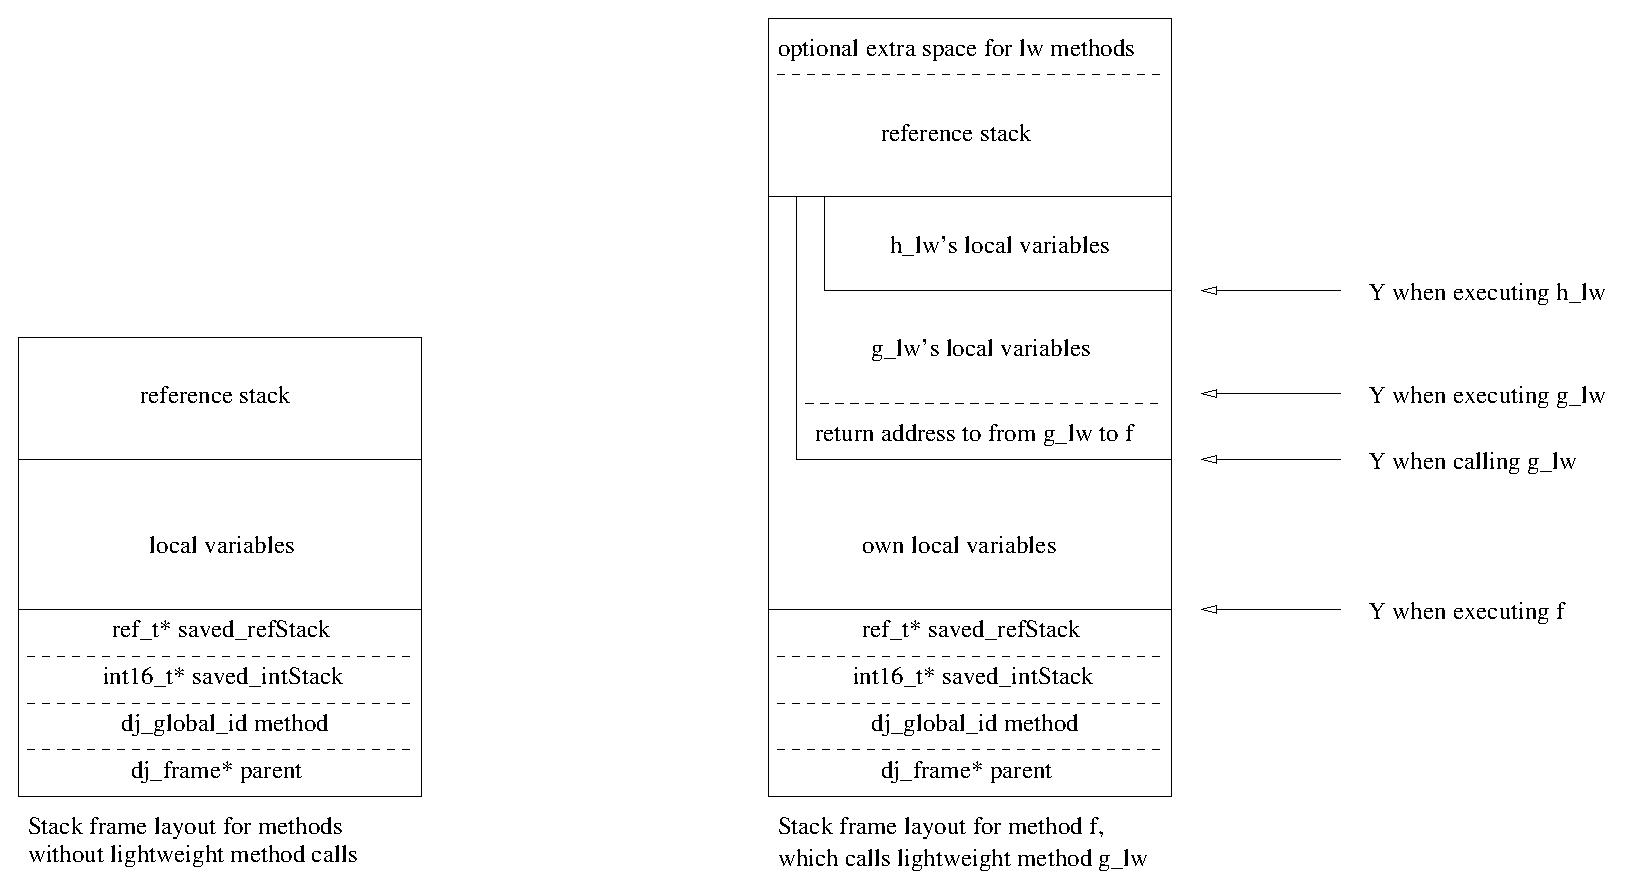
\includegraphics[width=0.95\linewidth]{stack-frame-lightweight-method.eps}
\caption{Stack frame layout for a normal method \mycode{f}, which calls lightweight method \mycode{g\_lw}, which in turn calls lightweight method \mycode{h\_lw}.}
\label{fig-stack-frame-lightweight-method}
\end{figure}

An example is shown in Figure \ref{fig-stack-frame-lightweight-method}, which shows the stack frame for a normal method \mycode{f}, which calls lightweight method \mycode{g\_lw}, which in turn calls another lightweight method \mycode{h\_lw}.

The stack frame for \mycode{f} contains space for its own locals, and for the locals of the lightweight method it calls: \mycode{g\_lw}. In turn, \mycode{g\_lw}'s locals contain space for \mycode{h\_lw}'s locals, as well as a slot to store the return address back to \mycode{f}. Since \mycode{h\_lw} does not call any other methods, it just keeps its return address in registers.

When a method calls a lightweight method with local variables, it will move the Y register to point at that method's locals. From Figure \ref{fig-stack-frame-lightweight-method} it is clear it only needs to increment Y by the size of its own locals. For \mycode{f}, this will place the Y register at the beginning of \mycode{g\_lw}'s locals. Since \mycode{g\_lw} may call \mycode{h\_lw}, \mycode{g\_lw}'s prologue will first store its return address in the first local slot, moving Y forward in the process so that Y points to the first free slot.

\subsubsection{Mark loop}
Lightweight methods may use any register and do not save call-saved registers like normal methods. The only case where this would be necessary is when it is called inside a \mycode{MARKLOOP} block that uses the same register to pin a variable. In this case we save those variables back to memory before calling the lightweight method and load them after the call returns. Since lightweight methods always come before their invocation in the infusion, the VM already knows which registers it uses, and will only save and restore pinned variables if there is a conflict. Because registers for mark loop are allocated low to high, and for normal stack caching from high to low, in many cases the two may not collide.

\subsubsection{Example call}
An example of the most complex case for a lightweight call is shown in Listing \ref{lst-full-lighweight-method-call}, which shows how method \mycode{f} from Figure \ref{fig-stack-frame-lightweight-method} would call \mycode{g\_lw}, assuming \mycode{f} is in a markloop block at the time which pinned a variable R14:R15, and these registers are also used by \mycode{g\_lw}.

In the translation of the \mycode{INVOKELIGHT} instruction we see we first flush the cache to memory, and then save the value of the local short at offset 22 that was pinned to R14:R15. Finally we add 26 to the Y register to skip the caller's own local variables and point Y to the start of the space reserved for lightweight method locals.

In the method call, we first see the return address is popped off the stack into a register. Since \mycode{g\_lw} may call another lightweight method, we cannot leave it there but store it in the first local slot, incrementing Y in the process. After \mycode{g\_lw} is done, we see the reverse process to return to the caller, where we then see the Y register is restored to point to the caller's locals, and the local variable at offset 22 is loaded back into the pinned register.

\begin{listing}
\centering
\begin{minipage}[t]{0.48\textwidth}
\begin{minted}{java}
// LIGHTWEIGHT INVOCATION
INVOKELIGHT g_lw
    push r25        // Flush the cache
    push r24
    std Y+22, r14   // Save pinned value
    std Y+23, r15
    adiw Y, 26      // Move Y to g_lw's
    call &g_lw                 // locals
    sbiw Y, 26      // Restore Y
    ldd r14, Y+22   // Reload pinned value
    ldd r15, Y+23
\end{minted}
\end{minipage}\hfill
\begin{minipage}[t]{0.48\textwidth}
\centering
\begin{minted}[linenos=false]{java}
// IMPLEMENTATION OF g_lw
    pop r18     // Pop the return address
    pop r19
    st Y+, r18  // Save in 1st local,
    st Y+, r19  //  and increment Y

      .. // g_lw's body

    ld r19, -Y  // Load return address,
    ld r18, -Y  //  and decrement Y
    push r19    // Push return address
    push r18    //  onto the stack
    ret
\end{minted}
\end{minipage}
\caption{Full lightweight method call}
\label{lst-full-lighweight-method-call}
\end{listing}


\subsection{Overhead comparison}
We now compare the overhead for the various ways we can call a method in Table \ref{tbl-method-invoke-overhead-comparison}.

Manually inlining code yields the best performance, but at the cost of increasing code size if larger methods are inlined. ProGuard inlining is currently slightly expensive because of the way it always saves parameters in local variables.

Both lightweight methods options cause some overhead, although this is very little compared to a full method call. First, we need to flush the stack cache to memory to make sure the parameters are on the real stack. This this takes two \mycode{push} and eventually two corresponding \mycode{pop} instructions per word, costing 8 cycles per word. In addition, we need to clear the value tags from the stack cache, which may mean we may not be able to skip as many \mycode{LOAD} instructions after the lightweight call, but this is hard to quantify.

Next the cost of translating the \mycode{INVOKE} instruction varies depending on the situation. In the simplest case it is simply a \mycode{CALL} to the lightweight method, which together with the corresponding \mycode{RET} costs 8 cycles. The worst case is 68 cycles when the lightweight method has local variables, uses all registers, and the caller used the maximum of 7 pairs to pin variables in a \mycode{MARKLOOP} block.

After calling the method, the method prologue for lightweight methods is very simple. We just need to save the return address and restore it in the epilogue, which takes 8 cycles if we can leave it in a register, or 16 if we need to store it in a local variable slot.

For small handwritten lightweight methods this is the only cost, but for larger ones created by converting a Java method, we add \mycode{STORE} instructions to copy the parameters from the stack into local variables, as shown in Listing \ref{lst-comparison-of-handwritten-and-converted-java-lw-method}. This is similar to the only overhead incurred by ProGuard's method inlining, and costs 4 cycles per word for the \mycode{STORE}, and possibly 4 more if the corresponding \mycode{LOAD} cannot be eliminated by popped value caching.

The total overhead for a lightweight method call scales nicely with the method's complexity. For the smallest methods, the minimum is only 16 cycles, plus 8 cycles per word for the parameters. For the most complex cases this may go up to 100 to 150 cycles. But these methods must be more complex and will have a longer run-time, so the relative overhead is still acceptable.

The number of cycles in Table \ref{tbl-method-invoke-overhead-comparison} is just a broad indication of the overhead. Some factors, such as the cost of clearing the value tags is hard to predict, and inlining may allow some optimisations that aren't possible with a method call. In practice the actual cost in a number of specific cases we examined varies, but is in the range we predicted.

Comparing this to a normal method call, we see the cost is much higher, and less dependent on the complexity of the method that is called. The overhead from setting up the stack frame, and the more expensive translation of the \mycode{INVOKE} instruction (see Listing \ref{lst-lightweight-stack-only}) are fixed, meaning a call will cost at least around 550 cycles, increasing to over 700 cycles for more complex methods taking many parameters.

%INVOKE COST FOR LIGHTWEIGHT METHOD:
%  8            CALL/RET
%  4            move Y
%  8 per word   saving markloop pinned registers used by lw method
%  0            pre/post invoke
%  0            setup callMethod parameters
%  
%  minimum: 8
%  maximum: 8 + 4 + 8*7 = 68
%  
%INVOKE COST FOR NORMAL METHOD:
%  8            CALL/RET
%  0            move Y
%  0            saving markloop pinned registers used by lw method
%  32+34        pre/post invoke
%  8            setup callMethod parameters
%  
%  total: 8+ = 82
\begin{table}
\caption{Approximate cycles of overhead caused by different ways of invoking a method}
\label{tbl-method-invoke-overhead-comparison}
	\centerline{
    \begin{tabular}{lccccc}
    \toprule
                                                              & Manual          & ProGuard                & Stack-only                  & Converted Java              & Normal                                              \\
                                                              & inlining        & inlining                & lightweight                 & lightweight                 & method call                                         \\
    \midrule
    \midrule
    flush the stack cache \footnote{excluding effect on future popped value cache performance because of cleared value tags}
                                                              &                 &                         & 8 per word                  & 8 per word                  & 8 per word                                          \\
    \mycode{INVOKE}                                           &                 &                         & 8 to 68                     & 8 to 68                     & \textasciitilde 82                                  \\
    create stack frame                                        &                 &                         &                             &                             & \textasciitilde 450                                 \\
    method pro-/epilogue                                      &                 &                         & 8 or 16                     & 8 or 16                     & 10 to 71                                            \\
    store and load parameters                                 &                 & 4 or 8 per word         &                             & 4 or 8 per word             & 4 or 8 per word                                     \\
    \\
    \emph{total}                                              &                 & \emph{4 or 8 per word}  & \emph{16 to 84 +}           & \emph{16 to 84 +}           & \emph{\textasciitilde 542 to \textasciitilde 603 +} \\
                                                              &                 &                         & \emph{8 per word}           & \emph{12 or 16 per word}    & \emph{12 or 16 per word}                            \\
    \bottomrule
    \end{tabular}
    }
\end{table}

\subsection{Creating lightweight methods}
We currently support two ways to create a lightweight method:
\begin{itemize}
	\item handwritten JVM bytecode
	\item converting a Java method 
\end{itemize}

\subsubsection{Handwritten JVM bytecode}
For the first option we declare the methods \mycode{native} in the Java source code, so the code calling it will compile as usual. We provide the infuser with a handwritten implementation in JVM bytecode, which the infuser will simply add to the infusion, and then process it in the same way as it processes a normal method, with one step added:

For lightweight methods, the parameters will be on the stack at the start of the method, but the infusers expects to start with an empty stack. To allow the infuser to process them like other methods, we add a dummy \mycode{LW\_PARAMETER} instruction for each parameter. This instruction is skipped when writing the binary infusion, but it tricks the infuser into thinking the parameters are being put on the stack.


\subsubsection{Converting Java methods}
This handwritten approach is useful for the smallest methods, and allows us to create bytecode that only uses the stack, which produces the most efficient code. But for more complex methods it quickly becomes very cumbersome to write the bytecode by hand.

As a second, slightly slower, but more convenient option, we developed a way to convert normal Java methods to lightweight methods by adding a \mycode{@Lightweight} annotation to it.

The infuser will scan all the methods in an infusion for this annotation. When it finds a method marked \mycode{@Lightweight}, the transformation to turn a normal JVM method into a lightweight one is simple: we first add a dummy \mycode{LW\_PARAMETER} instruction for each parameter, followed by \mycode{STORE} instructions to pop these parameters off the stack and store them in the right local variables. After this, we can use the normal body of the method and call it as a lightweight method.

Listing \ref{lst-comparison-of-handwritten-and-converted-java-lw-method} shows the difference for the \mycode{isOdd} method. We can see this approach adds some overhead in the form of a \mycode{SSTORE\_0} and a \mycode{SLOAD\_0} instruction. However, using popped value caching, only the \mycode{SSTORE\_0} will have a run-time cost. Another disadvantage of the converted method is that is has to use a local variable, which will slightly increase memory usage, but in return this approach gives us a very easy way to create lightweight methods.

\begin{listing}
 \centering
 \begin{minipage}[t]{0.32\textwidth}
  \centering
  \begin{minted}{java}
// JAVA
@Lightweight
public static boolean
          isOdd (short a)
{
  return (a & (short)1)==1;
}
  \end{minted}
 \end{minipage}\hfill
 \begin{minipage}[t]{0.29\textwidth}
  \centering
  \begin{minted}[linenos=false]{java}
// HANDWRITTEN
//              (Stack)
LW_PARAMETER    (Int)
SCONST_1        (Int,Int)
SAND            (Int)
SRETURN         ()
  \end{minted}
 \end{minipage}\hfill
 \begin{minipage}[t]{0.29\textwidth}
  \centering
  \begin{minted}[linenos=false]{java}
// CONVERTED JAVA
//              (Stack)
LW_PARAMETER    (Int)
SSTORE_0        ()
SLOAD_0         (Int)
SCONST_1        (Int,Int)
SAND            (Int)
SRETURN         ()
  \end{minted}
 \end{minipage}
 \vspace{0.5cm}

\caption{Comparison of hand written lightweight method and converted Java method}
\label{lst-comparison-of-handwritten-and-converted-java-lw-method}
\end{listing}


\subsubsection{Replacing \mycode{INVOKE}s}
The infuser does a few more transformations to the bytecode. Every method is scanned for \mycode{INVOKESTATIC} instructions that invoke a lightweight method. These are simply replaced by an \mycode{INVOKELIGHT}, and the number of extra slots for the reference stack and local variables of the current method is increased if necessary. Finally, methods are sorted so a lightweight method will be defined before it is invoked, to make sure the VM can always generate the \mycode{CALL} directly.


\subsection{Limitations and tradeoffs}
There are a few limitations to the use of lightweight methods:
\paragraph{No recursion} Since we need to be able to determine how much space to reserve in the caller's stack frame for a lightweight method's reference stack and local variables, we do not support recursion, although lightweight calls can be nested.

\paragraph{No garbage collection}
Lightweight methods reuse the caller's stack frame. This is a problem for the garbage collector, which works by inspecting each stack frame and finding the references on the stack and in local variables. If the garbage collector would be triggered while we're in a lightweight call, it would not know where to find the lightweight method's references, since the stack frame only has information for the method that owns it.

While it may be possible to relax this constraint with some effort, in most cases this is only a minor restriction. Lightweight methods are most useful for fast and frequently called methods, and operations that may trigger the garbage collector are usually expensive, so there is less to be gained from using a lightweight method in these situations.

\paragraph{Static only}
We currently do not support lightweight virtual methods, since the overhead of resolving the target of the invoke is large compared to the rest of the invoke overhead, but this is something that could be considered in future work.

\paragraph{Stack frame usage}
Finally, while many methods can be made lightweight, we should remember that a method calling a lightweight method will always reserve space for it in its locals. This space is reserved, regardless of whether the method is currently executing or not, and the more nested lightweight calls are made, the more space we need to reserve.

As an example if we have a method \mycode{f1} which may call a lightweight method with a large number of local variables, \mycode{big\_lw}, but is currently calling normal method \mycode{f2}, which may also call \mycode{big\_lw}, we will have reserved space for \mycode{big\_lw} twice, both in \mycode{f1}'s and in \mycode{f2}'s frame.

